\documentclass{article}
\usepackage{tikz}
\usepackage{amssymb}
\usepackage{amsmath}
\usepackage{xcolor}
\usetikzlibrary{calc, shapes, fit,arrows.meta}

\begin{document}

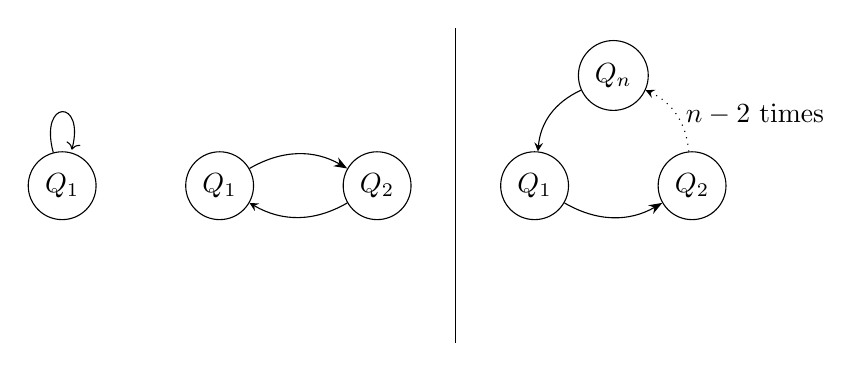
\begin{tikzpicture}
    \node (A) [draw = black, circle] at (0,0){$Q_1$};

    \draw  (A)edge [loop above](A);

    \node (B) [draw = black,circle] at (2,0){$Q_1$};
    \node (C) [draw = black,circle] at (4,0){$Q_2$};

    \draw (B) edge [bend left, arrows = -Stealth] (C);
    \draw (C) edge [bend left, arrows = -stealth] (B);

    \draw (5,2)--(5,-2);

    \node (D) [draw = black,circle] at (6,0){$Q_1$};
    \node (E) [draw = black,circle] at (8,0){$Q_2$};
    \node (F) [draw =black,circle] at  (7,1.4){$Q_n$};
    \draw (D) edge [bend right, arrows = -Stealth ] (E);
    \draw (E) edge [bend right, arrows = -stealth, dotted] node[right]{$n-2$ times} (F);
    \draw (F) edge [bend right, arrows = -stealth] (D);
\end{tikzpicture}

\end{document}